\documentclass[aps,prd,10pt,twocolumn,superscriptaddress,floatfix,nofootinbib,amsmath,amssymb,altaffilletter,preprintnumbers]{revtex4-1}
\usepackage[colorlinks=true,pdfstartview=FitV,breaklinks=true]{hyperref}


\usepackage[utf8]{inputenc}
\usepackage{graphicx}
\usepackage{booktabs}
\usepackage{tabularx}
\usepackage{textcomp}
\usepackage{xspace}
\usepackage{slashed}
\usepackage{amsmath}
\usepackage{amsfonts}
\usepackage{amssymb}
\usepackage{upgreek}
\usepackage{comment}
\usepackage[dvipsnames,table]{xcolor}
\usepackage[normalem]{ulem}
\usepackage{csquotes}
\usepackage{bbold}
%\usepackage[compat=1.1.0]{tikz-feynman}
%\usepackage{tikz}
\hypersetup{urlcolor=BlueViolet,
	    citecolor=Plum,
	    linkcolor=PineGreen}
\usepackage[official]{eurosym}
\definecolor{lightgray}{rgb}{0.9,0.9,0.9}	    
\definecolor{green}{rgb}{0,0.5,0}
\definecolor{red}{rgb}{1,0,0}
\definecolor{blue}{rgb}{0,0,0.5}

%\usepackage[right=2.5cm,left=2.5cm]{geometry}

\newcommand\codo[1]{{\tt #1}}
\newcommand{\n}{{\ensuremath{\mathfrak{n}}}\xspace} 
\newcommand{\comm}[1]{{\color{red} #1}}
\newcommand{\de}[1]{\partial #1}
\newcommand{\dt}[1]{\rm d #1}

\renewcommand{\arraystretch}{1.5}

\newcommand{\G}[1]{\textcolor{orange}{\textbf{GP:} #1}}
\newcommand{\Yeray}[1]{\textcolor{green}{\textbf{YG:} #1}}
\newcommand{\Yerayc}[1]{\textcolor{green}{#1}}

\DeclareMathOperator*{\sotimes}{\text{\raisebox{0.25ex}{\scalebox{0.6}{$\bigotimes$}}}}


\begin{document}

\title{Prospects for relic neutrino detection using nuclear spin experiments}

\author{Yeray Garcia del Castillo}\email{y.garcia\textunderscore del\textunderscore castillo@unsw.edu.au}
\author{Giovanni Pierobon}\email{g.pierobon@unsw.edu.au}
\author{Dipan Sengupta}\email{dipan.sengupta@unsw.edu.au}
\author{Yvonne Y. Y. Wong}\email{yvonne.y.wong@unsw.edu.au}
\affiliation{Sydney Consortium for Particle Physics and Cosmology\\
School of Physics, The University of New South Wales, Sydney NSW 2052,  Australia}

\preprint{CPPC-2025-06}


\onecolumngrid
\appendix


\section{Excitation and de-excitation rates}\label{app:rates}

\subsection{Single spin}

Consider first a single spin immersed in the cosmic neutrino bath.  Following Fermi's golden rule the excitation and de-excitation rates are given by 
\begin{equation}
\gamma_{\pm}=   |T^{\pm}_{\rm fi}|^2 
  2\pi\delta^{(1)}(E_{\rm f}-E_{\rm i}) \, \rho_\pm(E_{\rm f})\, ,
\label{eq:golden}
\end{equation}
where the superscripts ``$+$'' and ``$-$'' refer respectively to excitation and de-excitation, $|T^+_{\rm fi}|^2$ is the transition probability from the initial state $|{\rm i}\rangle = |\downarrow \rangle \otimes |{\rm i}_{\nu}\rangle$ to the final state $|{\rm f}\rangle= |\uparrow \rangle \otimes |{\rm f}_{\nu}\rangle$, while $|T^-_{\rm fi}|^2$ is its counterpart for the transition $|{\rm i}\rangle = |\uparrow \rangle \otimes |{\rm i}_{\nu}\rangle$ to $|{\rm f}\rangle= |\downarrow \rangle \otimes |{\rm f}_{\nu}\rangle$.  The quantity $\rho(E_{\rm f})$ is the density of states at the final energy $E_{\rm f}$, which in our case can be written as, 
\begin{equation}
\rho_\pm(E_{\rm f}) =  \sum_{jk} \sum_{a,c} \int \frac{{\rm d}^3\vec{p}}{(2 \pi)^3 }  \frac{{\rm d}^3 \vec{p}\,'}{(2 \pi)^3 } \frac{{\rm d}^3\vec{n}}{(2 \pi)^3 }   \, (2 \pi)^3 \delta^{(3)} ( \vec{p}-\vec{p}\,'\mp \vec{n})\, P_{{\rm i}_\nu} \, P_{{\rm f}_\nu}\,,
\label{eq:densityofstates}
\end{equation}
where $\vec{p}$ and $\vec{p}\,'$ are the 3-momenta of the incoming and outgoing neutrinos respectively, $\vec{n}$ is the momentum of the final-state fermion (assuming it is initially stationary),  $P_{{\rm i}_\nu}$ and $P_{{\rm f}_\nu}$ represent respectively the thermal weight of the initial-state neutrino and any Pauli blocking factor associated with the final state, $j$ and $k$ are mass indices of the initial- and final-state neutrinos, while $a$ and $c$ index their helicities.  
Since the recoil of the fermion is expected to be tiny, the angle of the outgoing neutrino is essentially unrestricted.  We therefore proceed to use the Dirac delta in Eq.~\eqref{eq:densityofstates} to eliminate the integral over the nuclear momentum, to arrive at
\begin{equation}
\rho_\pm(E_{\rm f}) =  \sum_{jk} \sum_{a,c} \int \frac{{\rm d}^3\vec{p}}{(2 \pi)^3 }  \frac{{\rm d}^3\vec{p}\,'}{(2 \pi)^3 }   P_{{\rm i}_\nu} \, P_{{\rm f}_\nu}\, ,
\label{eq:densityofstates2}
\end{equation}
where it is now understood that the relation between $|\vec{p}|$ and $|\vec{p}\,'|$ is determined by energy conservation alone.


%%%%%%%%%%%%%%%%%%%%%%%%%%%%%%%%
%%%%%%%%%%%%%%%%%%%%%%%%%%%%%
\begin{figure}
    \centering
    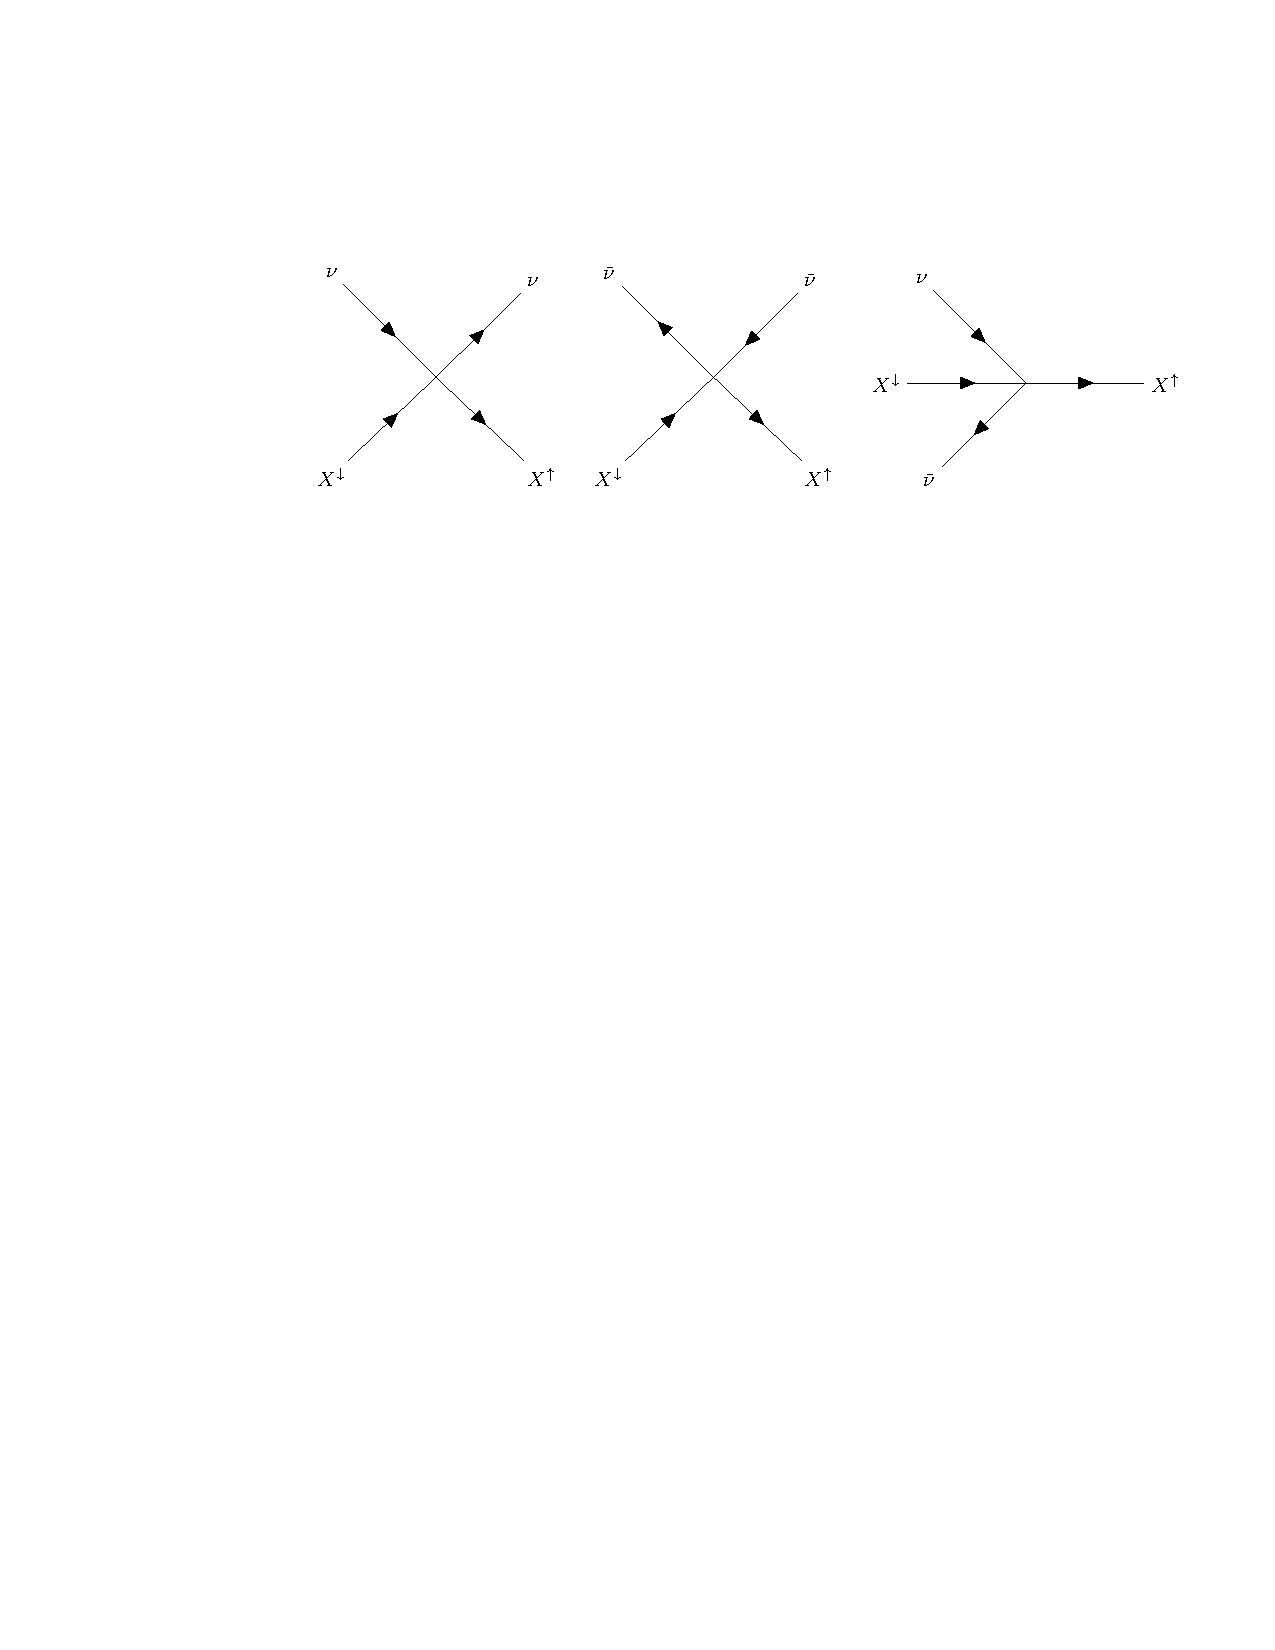
\includegraphics[width=0.9\linewidth]{../plots/diagram.pdf}
    \caption{Feynman diagrams of the processes that contribute to the excitation of a spin in a 4-fermi effective interaction.}
    \label{fig:feynman}
\end{figure}
%%%%%%%%%%%%%%%%%%%%%%%%%%%%%%%%%%%
%%%%%%%%%%%%%%%%%%%%%%%%%%%%%%%%%%%%%

At first order in perturbation theory (i.e., the Born approximation), the transition amplitude is given by 
\begin{equation}
    T^{\pm}_{\rm fi}=\langle {\rm f}|\Sigma_{\pm}J_{\pm}|{\rm i}\rangle \, .
\end{equation}
Focussing on excitation, consider an initial-state neutrino specified by a wavefunction 
\begin{equation}
\nu_j(t,\vec{x}) = u_{j,a}(\vec{p})  e^{-{\rm i} (p^0t-\vec{p}\cdot\vec{x})}\, ,
\end{equation}
where $a$ is a helicity index.  Suppose it scatters off a spin inelastically, thereby transferring energy $\omega_0$ to it, and then exits the interaction in a final-state plane wave given by $\nu_k(t,\vec{x}) = u_{k,c}(\vec{p}\,')  e^{-{\rm i}(p'^0t- \vec{p}' \cdot\vec{x})}$.  This process is represented by the leftmost diagram in Fig.~\ref{fig:feynman}, and its transition probability can be written as 
\begin{equation}
\begin{aligned}
    |T^{+}_{\rm fi}|^2= &\; |\langle \uparrow |J_{+}|\downarrow \rangle|^2\, |\langle {\rm f}_\nu | \Sigma_+ | {\rm i}_\nu \rangle|^2 \\
    =& \;   \, \frac{G_F^2}{2} g_A^{j,k} g_A^{k,j} \frac{1}{2p^{0}2p'^{0}}   \left| \bar{u}_{k,c}(\vec{p}\,') (\gamma^1 - {\rm i} \gamma^2)(1- \gamma^5) u_{j,a}(\vec{p})\right|^2\, ,
\end{aligned}
\end{equation}
where we have used $|\langle\uparrow|J_+|\downarrow \rangle|^2=1$ at the second equality, and the factors of $1/2 p^{0}$ originates from the normalisation of the $u$-spinors to $2p^0$.
The thermal weight factors in Eq.~\eqref{eq:densityofstates} are then $P_{{\rm i}_\nu} = N_{j,a}(p^0)$ and  $P_{{\rm f}_\nu} =1 -N_{k,a}(p'^0)$, where $N_{i,a}(p^0)$ is the neutrino occupation number, while the Dirac delta $\delta^{(1)}(E_{\rm f}-E_{\rm i})$ becomes $\delta^{(1)}(\omega_0+p'^0-p^0)$, 
enforcing the change in energy between the initial- and final-state neutrinos to be equal to $\omega_{0}$, the energy splitting due to the external magnetic field.   A similar calculation can also be performed in the case of an antineutrino exciting a spin, as represented by the middle diagram in Fig.~\ref{fig:feynman}.  



Putting it altogether, we then find the excitation rate of one spin to be
\begin{equation}
\begin{aligned}
\gamma_{+}= & \; G_F^2\pi \sum_{jk} g_A^{j,k} g_A^{k,j} \sum_{ac}  
    \int {\rm d} \tilde{p} \int {\rm d} \tilde{p}' \; \delta^{(1)}(\omega_0+p'^0-p^0) \\
  &\; \times \Bigg[(1-N_{k,c}(p'^0)) \, N_{j,a}(p^0)\, \bar{u}_{k,c}(\vec{p}\,') (\gamma^1- {\rm i} \gamma^2)(1-\gamma^5) u_{j,a}(\vec{p}) 
    \bar{u}_{j,a}(\vec{p}) (\gamma^1+ {\rm i} \gamma^2)(1-\gamma^5) u_{k,c}(\vec{p}\,') \\
&\; \qquad +(1-\bar{N}_{k,c}(p'^0))\, \bar{N}_{j,a}(p^0)\bar{v}_{j,a}(\vec{p}) (\gamma^1- {\rm i} \gamma^2)(1-\gamma^5) v_{k,c}(\vec{p}\,') \bar{v}_{k,c}(\vec{p}\,') (\gamma^1+ {\rm i} \gamma^2)(1-\gamma^5) v_{j,a}(\vec{p})  \Bigg]\,,
    \label{eq:rate1heuristic}
    \end{aligned}
\end{equation}
where we have defined the phase space measure ${\rm d} \tilde{p} \equiv {\rm d}^3\vec{p}/((2 \pi)^3 2 p^0)$.  Ignoring the relative motion between the spin and the C$\nu$B, and assuming the neutrino occupation numbers to be independent of helicity, the expression simplifies to 
\begin{equation}
\begin{aligned}
\gamma_{+}= & \;8  \, G_F^2 \pi \sum_{jk} g_A^{j,k} g_A^{k,j} 
    \int {\rm d} \tilde{p} \int {\rm d} \tilde{p}' \; \delta^{(1)}(\omega_0+p'^0-p^0) \, p^0 p'^0\, \left[(1-N_{k}(p'^0)) \, N_{j}(p^0)  +(1-\bar{N}_{k}(p'^0))\, \bar{N}_{j}(p^0)\right]\,,
    \end{aligned}
\end{equation}
which, using the Dirac delta, can be further reduced to 
\begin{equation}
    \gamma_{+}= \frac{4G_F^2}{(2 \pi)^3} \sum_{jk} g_A^{j,k} g_A^{k,j}  
    \int_{\sqrt{(\omega_0+m_k)^2-m_j^2}}^\infty  {\rm d} |\vec{p}|\;|\vec{p}|^2\, p_{k+}\, \sqrt{m_k^2+p^2_{k+}} \,  
    \left[(1-N_{k}(p^0_{k+})) \, N_{j}(p^0)  +(1-\bar{N}_{k}(p^0_{k+}))\, \bar{N}_{j}(p^0)\right]\,,
    \label{eq:gamma+heuristic}
\end{equation}
with $p_{k+}=[(\sqrt{|\vec{p}|^2+m_j^2}-\omega_0)^2-m_k^2]^{1/2}$, and  $p^0_{k+}=\sqrt{m_k^2+p^2_{k+}}$.


Computation of the de-excitation rate from inelastic neutrino-spin scattering proceeds in a similar fashion, and yields
\begin{equation}
\begin{aligned}
\gamma_{-}= & \; G_F^2\pi \sum_{jk} g_A^{j,k} g_A^{k,j} \sum_{ac}  
    \int {\rm d} \tilde{p} \int {\rm d} \tilde{p}' \; \delta^{(1)}(\omega_0+p^0-p'^0) \\
  &\; \times \Bigg[(1-N_{k,c}(p'^0)) \, N_{j,a}(p^0)\, \bar{u}_{k,c}(\vec{p}\,') (\gamma^1+ {\rm i} \gamma^2)(1-\gamma^5) u_{j,a}(\vec{p}) 
    \bar{u}_{j,a}(\vec{p}) (\gamma^1- {\rm i} \gamma^2)(1-\gamma^5) u_{k,c}(\vec{p}\,') \\
&\; \qquad +(1-\bar{N}_{k,c}(p'^0))\, \bar{N}_{j,a}(p^0)\bar{v}_{j,a}(\vec{p}) (\gamma^1+ {\rm i} \gamma^2)(1-\gamma^5) v_{k,c}(\vec{p}\,') \bar{v}_{k,c}(\vec{p}\,') (\gamma^1- {\rm i} \gamma^2)(1-\gamma^5) v_{j,a}(\vec{p})  \Bigg]\,.
    \label{eq:rate2heuristic}
    \end{aligned}
\end{equation}
Again, ignoring any neutrino-spin relative motion and assuming  helicity-independent neutrino occupation numbers, we find
\begin{equation}
\begin{aligned}
\gamma_{-}= & \;8  \, G_F^2 \pi \sum_{jk} g_A^{j,k} g_A^{k,j} \sum_{ac}  
    \int {\rm d} \tilde{p} \int {\rm d} \tilde{p}' \; \delta^{(1)}(\omega_0+p^0-p'^0) \, p^0 p'^0\, \left[(1-N_{k}(p'^0)) \, N_{j}(p^0)  +(1-\bar{N}_{k}(p'^0))\, \bar{N}_{j}(p^0)\right] \\
    =&\;  \frac{4G_F^2}{(2 \pi)^3} \sum_{jk} g_A^{j,k} g_A^{k,j}  
    \int_{\sqrt{(\omega_0-m_k)^2-m_j^2}}^\infty  {\rm d} |\vec{p}| \;|\vec{p}|^2\, p_{k-}\, \sqrt{m_k^2+p^2_{k-}} \,  
    \left[(1-N_{k}(p^0_{k-})) \, N_{j}(p^0)  +(1-\bar{N}_{k}(p^0_{k-}))\, \bar{N}_{j}(p^0)\right]\,,
    \label{eq:gamma-heuristic}
    \end{aligned}
\end{equation}
with  $p_{k-}=[(\sqrt{|\vec{p}|^2+m_j^2}+\omega_0)^2-m_k^2]^{1/2}$, and $p^0_{k-}=\sqrt{m_k^2+p^2_{k-}}$.    The lower integration holds if it evaluates to a real number.  Otherwise, it needs to be set to zero. 


Suppose for simplicity $m_j = m_k=m$ and $\omega_0 \ll m$.  The lower integration limits of the $\gamma_+$ and $\gamma_-$ integrals, Eqs.~\eqref{eq:gamma+heuristic} and~\eqref{eq:gamma-heuristic}, are $\sqrt{(\omega_0+m)^2-m^2} \approx \sqrt{2 m\omega_0}$ and zero, respectively.  We can take the former to zero too if $\omega_0 \ll |\vec{p}|^2/(2 m) \ll m$ is satisfied by the bulk of the neutrino distribution.  The same condition also allows us to approximate $p_{k\pm} \approx \sqrt{ |\vec{p}|^2\mp 2m \omega_0}\approx|\vec{p}| \mp m\omega_0/|\vec{p}|$. Then, to leading order, we find 
\begin{equation}
\begin{aligned}
\gamma_+ \approx \gamma_- & \propto \int_0^\infty {\rm d}|\vec{p}|\; |\vec{p}|^2 \; p_{k+}\sqrt{m^2+p^2_{k+}}  \left[N(p^0) + \bar{N}(p^0)\right] \\
& \approx \int_0^\infty {\rm d}|\vec{p}|\; |\vec{p}|^2\;  m \, |\vec{p}|  \left[N(p^0) + \bar{N}(p^0)\right] \, ,
\end{aligned}
\end{equation}
and
\begin{equation}
\begin{aligned}
\gamma_{\rm net} \equiv \gamma_--\gamma_+&  \propto \int^\infty_0 {\rm d}|\vec{p}| \; |\vec{p}|^2\; \left[p_{k-}\, \sqrt{m^2+p^2_{k-}}- p_{k+}\, \sqrt{m^2+p^2_{k+}}
\right] \left[N(p^0) + \bar{N}(p^0)\right] \\
& \approx   \int^\infty_0 {\rm d}|\vec{p}| \; |\vec{p}|^2\; \frac{2 m^2 \omega_0}{|\vec{p}|} \; \left[N(p^0) + \bar{N}(p^0)\right] \, ,
\end{aligned}
\end{equation}
where we have omitted for brevity the Pauli-blocking terms in both expressions.  Thus, we see immediately that $\gamma_{+}< \gamma_-$, and $\gamma_{\rm net}$ is suppressed by a factor $\sim 2 m \omega_0/|\vec{p}|^2$ relative to $\gamma_\pm$.

%%%%%%%%%%%%%%% 
%%%%%%%%%%%%%%%

\subsection{\texorpdfstring{$N$}{N} spins}

Consider now a system of $N$ spins described by the interaction Hamiltonian~\eqref{eq:nham}.  We are interested in the excitation and de-excitation rates of the whole spin ensemble, which can be defined via
\begin{equation}
\Gamma_\pm = \sum_{{\rm f}_{\rm spin}}|T_{\rm fi}^{\pm}|^2
2 \pi \delta^{(1)}(E_{\rm f}-E_{\rm i})\, \rho_\pm (E_{\rm f})\, ,
\label{eq:Gammapm}
\end{equation}
where 
\begin{equation}
\begin{aligned}
T^{\pm}_{\rm fi} = &\; \sum_\alpha \langle {\rm f}_{\rm spin} |  J_\pm^\alpha |{\rm i}_{\rm spin}\rangle \langle {\rm f}_\nu | \Sigma_\pm^\alpha | {\rm i}_\nu \rangle
\end{aligned}
\end{equation}
are the excitation and de-excitation amplitudes of the $N$-spin ensemble from an initial state $|{\rm i}_{\rm spin} \rangle$ to an unspecified final state $|{\rm f}_{\rm spin} \rangle$. The summation over ${\rm f}_{\rm spin}$ encompasses a complete basis of  final states; the ladder operators will project out the final states that have one unit of energy $\omega_0$ more ($+$) or less ($-$) than the initial state.  


Again, focussing first on spin excitation due to inelastic scattering of a plane-wave neutrino from $\nu_j(t,\vec{x}_\alpha) = u_{j,a}(\vec{p})  e^{-{\rm i} (p^0t-\vec{p}\cdot\vec{x}_\alpha)}$ to $\nu_k(t,\vec{x}_\beta) = u_{k,c}(\vec{p}\,')  e^{-{\rm i} (p'^0t-\vec{p}\,'\cdot\vec{x}_\beta)}$, we find
\begin{equation}
\begin{aligned}
 |T^{+}_{\rm fi} |^2 = &\;  \sum_{\alpha \beta} \langle {\rm f}_{\rm spin}|  J_+^\alpha |{\rm i}_{\rm spin}\rangle
 \langle {\rm i}_{\rm spin}|  J_-^\beta |{\rm f}_{\rm spin} \rangle \\
 &\qquad \times \frac{G_F^2}{2} g_A^{j,k} g_A^{k,j}  \frac{1}{2p^{0}2p'^{0}} \left| \bar{u}_{k,c}(\vec{p}\,') (\gamma^1 - {\rm i} \gamma^2)(1- \gamma^5) u_{j,a}(\vec{p})\right|^2\, e^{-{\rm i}(\vec{p}\,' -\vec{p})\cdot(\vec{x}_\alpha-\vec{x}_\beta)} \, .
    \end{aligned}
    \end{equation}
A similar expression can be found for $|T^{-}_{\rm fi}|^2$.
Then, following the same procedure as for a single spin, it is straightforward to arrive at the collective excitation and  de-excitation rates
\begin{equation}
\begin{aligned}
\Gamma_{+}
    =&\;\frac{2G_F^2}{(2 \pi)^3} \sum_{jk} g_A^{j,k} g_A^{k,j}  
    \int_{\sqrt{(\omega_0+m_k)^2-m_j^2}}^\infty  {\rm d} |\vec{p}| \; |\vec{p}|^2\, p_{k+}\, \sqrt{m_k^2+p^2_{k+}} \,  
    \left[(1-N_{k}(p^0_{k+})) \, N_{j}(p^0)  +(1-\bar{N}_{k}(p^0_{k+}))\, \bar{N}_{j}(p^0)\right]\\
    &\; \hspace{30mm} \times\int_{-1}^1 {\rm d} \mu \; F_+(\vec{p}_{k+}-\vec{p})\, , \\
\Gamma_{-}= &\;\frac{2G_F^2}{(2 \pi)^3} \sum_{jk} g_A^{j,k} g_A^{k,j}  
    \int_{\sqrt{(\omega_0-m_k)^2-m_j^2}}^\infty  {\rm d} |\vec{p}|\; |\vec{p}|^2\, p_{k-}\, \sqrt{m_k^2+p^2_{k-}} \,  
    \left[(1-N_{k}(p^0_{k-})) \, N_{j}(p^0)  +(1-\bar{N}_{k}(p^0_{k-}))\, \bar{N}_{j}(p^0)\right]\\
    &\; \hspace{30mm} \times\int_{-1}^1 {\rm d} \mu \; F_-(\vec{p}_{k-}-\vec{p})\, ,
    \label{eq:BigGamma}
    \end{aligned}
\end{equation}
where $\mu \equiv \hat{p}' \cdot \hat{p}=\cos\theta_{\vec{p}\vec{p}\,'}$, with $\theta_{\vec{p}\vec{p}\,'}$ the angle between the incoming and outgoing momenta, and
\begin{equation}
F_\pm(\vec{p}\,'-\vec{p}) \equiv \sum_{\rm f_{spin}}\Big|\langle {\rm f}_{\rm spin}| \sum_\alpha  J_\pm^\alpha e^{-{\rm i} (\vec{p}\,' - \vec{p}) \cdot\vec{x}_\alpha}|{\rm i}_{\rm spin}\rangle \Big|^2
\label{eq:formfactors}
\end{equation}
are form factors that depend on the initial state of the whole $N$ spin ensemble.
 Since the operator $ \sum_\alpha  J_\pm^\alpha$ already projects the initial state into the subspace of final states that has the correct energy requirements,  we can use the completeness relation of all possible final states $\sum_{\rm f'_{spin}}|{\rm f'}_{\rm spin}\rangle\langle {\rm f'}_{\rm spin}|=1$ to simplify the form factors to
\begin{equation}
 F_\pm(\vec{p}\,'-\vec{p}) = \langle {\rm i}_{\rm spin}| \sum_\beta  J_\mp^\beta e^{+{\rm i} (\vec{p}\,' - \vec{p})\cdot \vec{x}_\beta} \sum_\alpha  J_\pm^\alpha e^{-{\rm i} (\vec{p}\,' - \vec{p}) \cdot \vec{x}_\alpha}|{\rm i}_{\rm spin}\rangle \,,
\label{eq:formfactorsAA}
\end{equation}
where it is understood that $F_\pm(\vec{p}\,'-\vec{p})$ are to be evaluated for $\vec{p}\,'=\vec{p}_{k+}$ or $\vec{p}\,'=\vec{p}_{k-}$.


Suppose the spin ensemble is initially in the ground state, i.e., $|{\rm i}_{\rm spin} \rangle = |\downarrow_1,\downarrow_2,\cdots,\downarrow_\gamma, \cdots, \downarrow_N \rangle$.   We see immediately that the de-excitation form factor must always yield $F^G (\vec{p}\,'-\vec{p})=0$, while the excitation form factor evaluates to
\begin{equation}
 F^G_+(\vec{p}\,'-\vec{p}) = \langle\downarrow_1,\downarrow_2, \cdots, \downarrow_N | \sum_\beta  J_-^\beta e^{+{\rm i} (\vec{p}\,' - \vec{p})\cdot \vec{x}_\beta} \sum_\alpha  J_+^\alpha e^{-{\rm i} (\vec{p}\,' - \vec{p})\cdot \vec{x}_\alpha}|\downarrow_1,\downarrow_2, \cdots, \downarrow_N \rangle=N\, ,
\end{equation}
irrespective of the momentum transfer. Thus, in this case there is no coherent effect from the neutrino-spin interaction.  If, on the other hand, the spin ensemble is initially in the product state $|{\rm i}_{\rm spin} \rangle = |\rightarrow_1, \rightarrow_2, \cdots, \rightarrow_\gamma, \cdots, \rightarrow_N \rangle$, where $|\rightarrow \rangle \equiv (|\uparrow \rangle + |\downarrow \rangle)/\sqrt{2}$, then the excitation and de-excitation form factors evaluate to
\begin{equation}
\begin{aligned}
 F^P_\pm(\vec{p}\,'-\vec{p}) & = \langle \rightarrow_1,\rightarrow_2, \cdots, \rightarrow_N | \sum_\beta  J_\mp^\beta e^{+{\rm i} (\vec{p}\,' - \vec{p})\cdot \vec{x}_\beta} \sum_\alpha  J_\pm^\alpha e^{-{\rm i} (\vec{p}\,' - \vec{p})\cdot \vec{x}_\alpha} |\rightarrow_1,\rightarrow_2, \cdots, \rightarrow_N \rangle\\
 & =\frac{N}{2}+\frac{1}{4}\sum_{\alpha, \beta \neq \alpha} e^{-{\rm i} (\vec{p}\,' - \vec{p})\cdot (\vec{x}_{\alpha}-\vec{x}_\beta)}\, ,
\end{aligned}
\end{equation}
which features possible coherent effects in the second term.  When the spatial separation between spins $|\vec{x}_{\alpha}-\vec{x}_\beta|$ is much smaller than $V^{1/3}$, where $V$ is the volume of the sample, we can take the continuum limit and, for a constant spin density $n_s=N/V$, approximate the last expression as
\begin{equation}
\begin{aligned}
F^P_\pm(\vec{p}\,'-\vec{p}) &= \frac{N}{2} +\frac{N^2}{4 V^2} \left| \int {\rm d}^3 x \; e^{{\rm i}(\vec{p}\,'-\vec{p})\cdot\vec{x}} \right|^2 \\
&= \frac{N}{2} + \frac{N^2}{4} \frac{9}{|\vec{p}\,'-\vec{p}|^2 R^2} \left|j_1\left(|\vec{p}\,'-\vec{p}| R\right) \right|^2\, ,
\label{eq:formP}
\end{aligned}
\end{equation}
where $j_1(x)$ is the spherical Bessel function of order one, and we have assumed at the second equality the spin sample to be a sphere of radius $R$.  Clearly, the second, $N^2$ term dominates if $|\vec{p}-\vec{p}\,'|R\ll1$,  with $|j_1(x)|^2/x^2 \to 1/9$ as $x \to 0$.
In this limit, the system exhibits coherent behaviours. 

Given the typical momentum of the neutrino bath $\vec{p}_\nu$, in order for the coherence condition to hold over the whole length $R$ of the spin sample, we must demand $|\vec{p}_\nu-\vec{p}\,'(\vec{p}_\nu)|R\ll1$. Assuming for simplicity $m_i=m_j=m$, the typical momentum transfers during excitation and de-excitation are 
\begin{equation}
    |\vec{p}_\nu-\vec{p}\,'(\vec{p}_\nu)|^2_\pm=p_\nu^2+(\sqrt{p_\nu^2+m^2}\mp\omega_0)^2-m^2-2p_\nu\left[(\sqrt{p_\nu^2+m^2}\mp\omega_0)^2-m^2\right]^{1/2}\cos{\theta_{\vec{p}\vec{p}\,'}}\,,
    \label{eq:co}
\end{equation}
with $p_{\nu} \equiv|\vec{p}_{\nu}|$.
 If we want coherence over the whole object, we must demand that $|\vec{p}_\nu-\vec{p}\,'(\vec{p}_\nu)|^2 \ll 1/R^2$ even for $\cos \theta_{\vec{p}\vec{p}\,'} = -1$.  
For non-relativistic neutrinos, where $\sqrt{p_\nu^2+m^2} \approx m + p_\nu^2/(2 m)$, 
this yields the condition
\begin{equation}
    p_\nu^2+(m+\epsilon_\pm)^2-m^2+2p_\nu\sqrt{(m+\epsilon_\pm)^2-m^2}\ll1/R^2\,,
\end{equation}
or, equivalently,
\begin{equation}
    p_\nu+\sqrt{(m+\epsilon_\pm)^2-m^2}\ll1/R\,,
    \label{eq:co2}
\end{equation}
with $\epsilon_\pm \equiv p_\nu^2/(2m) \mp \omega_0$.  This in turn leads to
\begin{equation}
    p_\nu \left[1+ \sqrt{1\mp \omega_0 \frac{2 m}{p_\nu^2}} \right]\ll1/R\,,
    \label{eq:co3}
\end{equation}
when expanded to linear order in $\epsilon_\pm$.

From Eq.~\eqref{eq:co3}, we see that excitation can only happen if $\omega_0< p_\nu^2/(2m)$.  But, if excitation happens at all, the coherence condition is also automatically fulfilled for any incoming momentum satisfying $p_\nu R\ll 1$. 
On the other hand, while de-excitation has no kinematic threshold, coherence also does not come for free. Rather, in order to have coherent de-excitation, the condition  $\omega_0\ll p_\nu^2/(2m)$ must be satisfied if $p_\nu R \ll 1$.  Physically, this means that the energy splitting must be much smaller than the incoming neutrino kinetic energy. If this is not the case, the momentum transfer of the neutrino is large and coherence is lost.    For a typical C$\nu$B momentum of $p_\nu \sim 5.3 \times 10^{-4}~{\rm eV} \sim 27~{\rm cm}^{-1}$ and a neutrino mass of $m=0.05$~eV, this condition amounts to demanding that $\omega_0 \ll 3 \times 10^{-6}$~eV. 

For typical spin samples of size $R \sim 1$~cm, the condition $p_\nu R \ll 1$ cannot be realised by the C$\nu$B across the whole sample volume. However, even in the case of $p_\nu R \gg1$, coherence is still possible under limited conditions.  Specifically, assuming $\omega_0\ll p_\nu^2/(2m)$, Eq.~\eqref{eq:co} evaluates to 
\begin{equation}
    |\vec{p}_\nu-\vec{p}\,'(\vec{p}_\nu)|^2\approx4p_\nu^2\sin^2{\frac{\theta_{\vec{p}\vec{p}\,'}}{2}}\,.
\end{equation}
Demanding $|\vec{p}_\nu-\vec{p}\,'(\vec{p}_\nu)|^2R^2 \ll 1$, we see that 
 coherence can be achieved even in the case $p_\nu R \gg 1$ for small angles $\theta_{\vec{p}\vec{p}\,'}\ll1/(p_\nu R)$ between the incoming and outgoing neutrino momenta. Under this condition, we can approximate the coherent part of the form factors as
\begin{equation}
\int_{-1}^1 {\rm d} \mu\; F_\pm^P(\vec{p}\,'-\vec{p}) \approx \frac{N^2}{4} \int_0^{(p_\nu R)^{-1}} {\rm d} \theta_{\vec{p}\vec{p}\,'}\, \sin\theta_{\vec{p}\vec{p}\,'} \approx \frac{N^2}{4} \frac{1}{2(p_\nu R)^{2}} \, .
\end{equation}
In other words, the collective excitation and de-excitation rates $\Gamma_\pm$ in the $p_\nu R \gg 1$ regime are suppressed by a factor $(2 p_\nu R)^{-2}$ relative to the fully coherent rates.  Evaluating Eq.~\eqref{eq:co} for the momentum transfer squared $q^2 \equiv|\vec{p}_\nu-\vec{p}\,'(\vec{p}_\nu)|^2$ in the forward direction (i.e., $\cos{\theta_{\vec{p}\vec{p}\,'}} = 1$) and expanding in $\epsilon_\pm$ as above, it is straightforward to show that the momentum transfer in this regime is $q \sim \omega_0 m/p_\nu$. 



\end{document}